\chapter[Model Evaluation]{Model Evaluation}

\begin{objetivos}
By the end of this chapter, readers should be able to:
\begin{itemize}
\item distinguish fit, discrimination, calibration, and transferability;
\item explain why random partitions may be optimistic;
\item choose among random, spatial, environmental, and independent validation;
\item interpret AUC, TSS, Kappa, sensitivity, specificity, and Boyce Index;
\item critically evaluate thresholds and binary maps; and
\item compare models without reducing the decision to a metric ranking.
\end{itemize}
\end{objetivos}

\section{Introduction}

Model evaluation is essential in SDM. A visually plausible map may still have
weak discrimination, sensitivity, specificity, or independence from calibration
data. Whenever possible, models should be evaluated using independent data
\parencite{fielding1997review,allouche2006assessing,hirzel2006evaluating,li2013thresholds,guisan2017habitat}.
Here, GLM, GAM, Random Forest, BRT, Maxent, and Ensemble predictions for
\textit{Dinizia excelsa} are compared to understand their performance,
limitations, and ecological coherence rather than automatically select the
largest metric.

\begin{conceito}[title={\faBook\quad Evaluation is not merely ranking}]
A useful SDM requires predictive performance, ecological coherence,
interpretable responses, and spatial or temporal generalization. The largest
AUC alone is not a sufficient decision rule.
\end{conceito}

\section{What Does It Mean to Evaluate an SDM?}

Evaluation confronts predictions with data not used to estimate model
parameters. Four questions follow. Does the model rank presences above absences
or background? When probabilistic interpretation is justified, do predicted
values agree with observed frequencies? Does error remain acceptable in a new
region, period, or environmental domain? Does the test design represent the
intended model use?

These questions concern \textbf{discrimination}, \textbf{calibration},
\textbf{transferability}, and \textbf{alignment between validation design and
prediction objective}. Good discrimination can coexist with poor calibration;
strong interpolation can coexist with failed transfer
\parencite{vaughan2005testing,jimenezvalverde2013discrimination,roberts2017crossvalidation}.

\begin{atencao}[title={\faExclamationTriangle\quad Suitability is not automatically probability}]
Probabilistic calibration is meaningful only when model output and sampling
design support occurrence or occupancy probability. Presence--background scores
do not become probabilities merely because they range from zero to one.
\end{atencao}

\section{Random Validation and Spatial Dependence}

Random cross-validation can place nearby records in training and test sets.
Neighboring locations often share climate, soil, sampling history, and residual
autocorrelation, making the test artificially easy and error estimates
optimistic \parencite{roberts2017crossvalidation}. This is particularly relevant
for Amazonian records clustered along rivers, roads, cities, and historically
surveyed sites.

\begin{conceito}[title={\faBook\quad Spatial leakage}]
Spatial leakage occurs when proximity, dependence, or shared sampling units let
training information make the test set artificially easy. A formally distinct
test record may still fail to provide independent information.
\end{conceito}

\section{Partitioning Strategies}

\subsection{Random Cross-Validation}
Useful for diagnosing fit within the sampled domain and comparing implementations
under a common split, but insufficient evidence of spatial transfer for
structured data.

\subsection{Spatial Blocks}
Whole geographic blocks are assigned to training or testing. Block size should
reflect autocorrelation, occurrence density, and prediction distance. Blocks
that are too small retain dependence; overly large blocks yield few,
imbalanced folds and variable error estimates
\parencite{roberts2017crossvalidation,valavi2019blockcv}.

\subsection{Buffering and Distance Separation}
Buffers exclude training records near test points and directly impose a minimum
calibration--evaluation distance, at the cost of smaller training sets and
potentially greater fold-to-fold variability.

\subsection{Environmental Blocking}
Records are grouped in environmental space, for example by clustering continuous
predictors. This tests transfer to environmental combinations not represented in
training and answers a different question from geographic blocking
\parencite{valavi2019blockcv}.

\subsection{Independent Validation}
Data from another campaign, region, or period provide the most direct test of
the corresponding transfer, provided definitions, effort, and detectability are
comparable. Geographic independence alone does not correct protocol differences.

\begin{atencao}[title={\faExclamationTriangle\quad No partition is universally best}]
The strategy must emulate intended use. Landscape interpolation, geographic
transfer, and future climate projection are different problems requiring
different tests.
\end{atencao}

\section{Reproducible Spatial Folds}

For \textit{Dinizia excelsa}, presences and background are linked to a grid in a
metric projection. Whole cells, not individual records, are assigned to folds.
Every fold must retain both classes, and spatial separation must represent a
relevant prediction distance.

\begin{rcode}
# Run from the project root
source("scripts/unidade12/09_criar_folds_espaciais.R")
source("scripts/unidade12/10_validacao_espacial_glm.R")
\end{rcode}
\rscriptref{scripts/unidade12/09_criar_folds_espaciais.R}
\rscriptref{scripts/unidade12/10_validacao_espacial_glm.R}

The first script writes fold assignments, the spatial grid, and a diagnostic
map. The second recalculates predictor standardization using training data only,
refits the GLM in each fold, and computes AUC, TSS, sensitivity, specificity,
and Brier score. Reusing means and standard deviations calculated from all
records would constitute preprocessing leakage.

\begin{atencao}[title={\faExclamationTriangle\quad Block size is not a decorative hyperparameter}]
The initial 300-km value is an explicit diagnostic setting, not a universal
recommendation. Final analysis should justify distance using the question's
scale, sampling pattern, autocorrelation, and transfer horizon.
\end{atencao}

\begin{figure}[htbp]
\centering
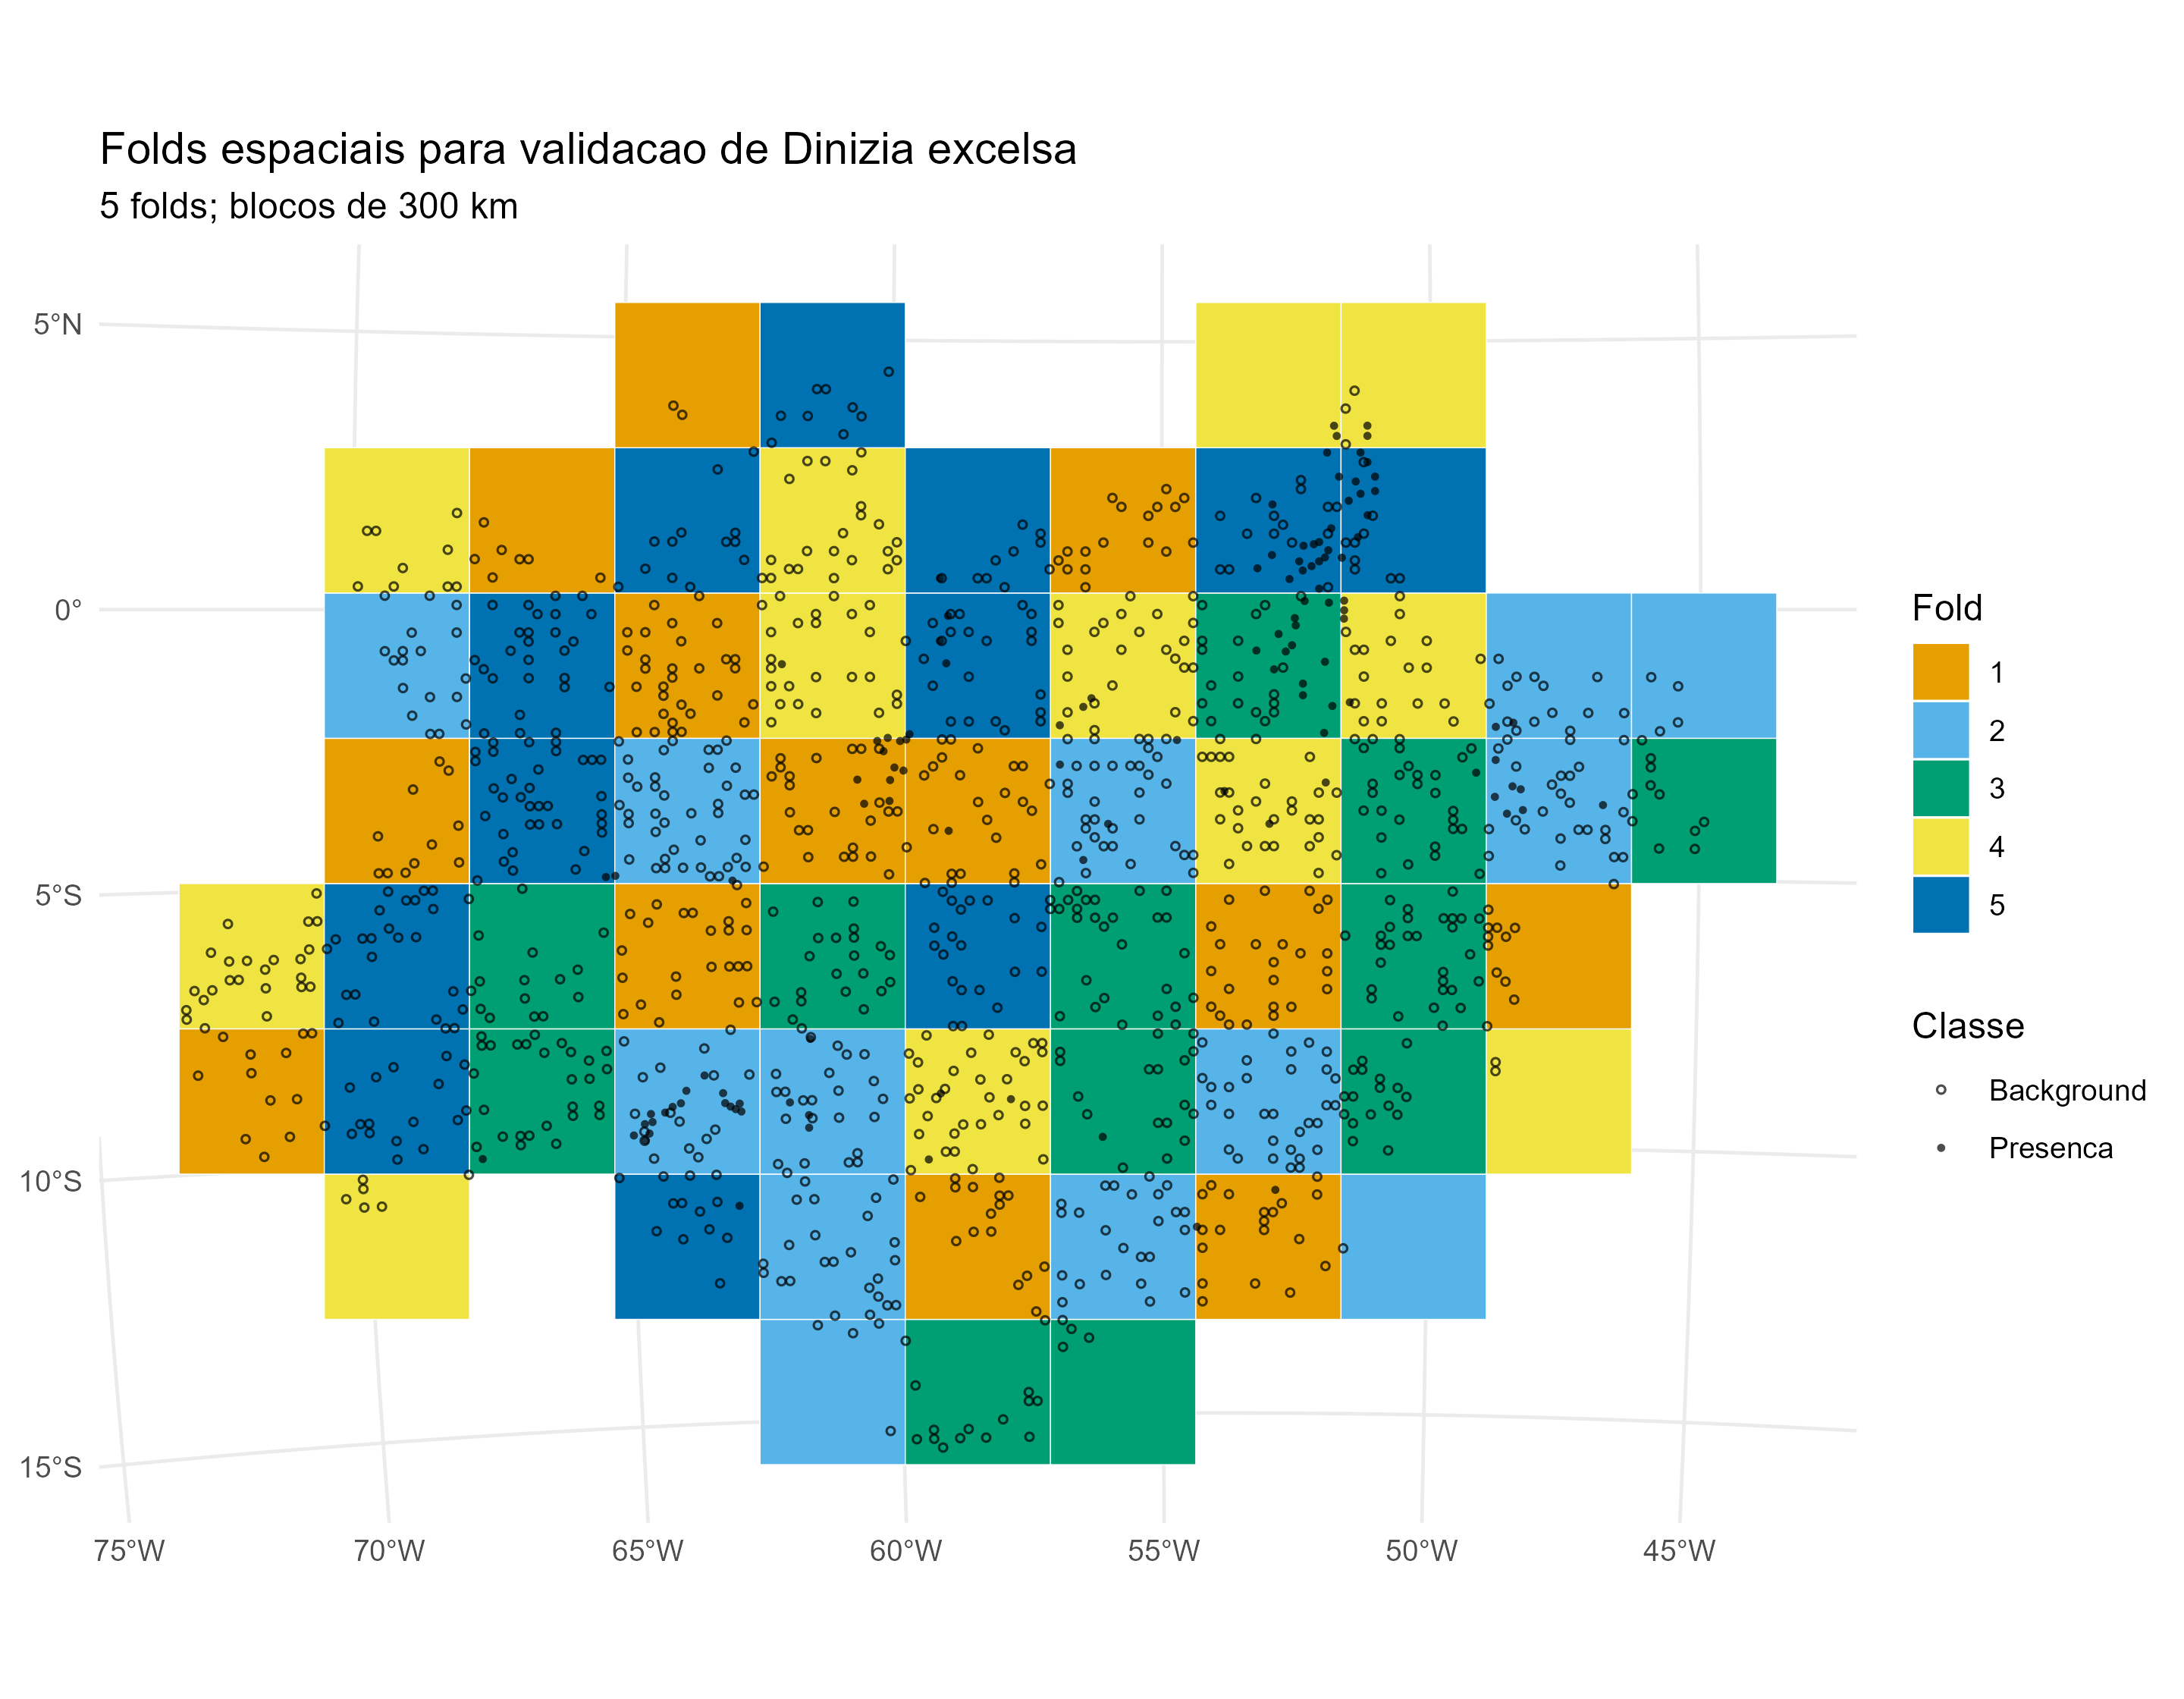
\includegraphics[width=0.93\textwidth]{figuras/unidade12/unidade12_folds_espaciais.png}
\caption{Reproducible spatial partition used for diagnosis. Each 300-km cell belongs entirely to one of five folds; filled circles are presences and open circles are background. Cells from one fold may be dispersed, so this configuration does not impose an exclusion buffer between training and testing.}
\label{fig:unidade12-folds-espaciais}
\end{figure}

\subsection{Spatial Diagnostic Results}
All folds retained presences and background. The GLM converged in all refits,
but AUC ranged from 0.643 to 0.851 and specificity from 0.475 to 0.829. This
variation is more informative than a single average because it reveals unstable
regional transfer.

\begin{table}[htbp]
\centering
\caption{GLM performance across five spatial folds. Mean and standard deviation (SD) summarize independent refits.}
\label{tab:unidade12-validacao-espacial}
\begin{tabular}{lrrr}
\toprule
Metric & Mean & SD & Range \\
\midrule
AUC & 0.779 & 0.082 & 0.643--0.851 \\
TSS & 0.528 & 0.093 & 0.419--0.658 \\
Sensitivity & 0.826 & 0.132 & 0.632--0.944 \\
Specificity & 0.703 & 0.155 & 0.475--0.829 \\
Brier & 0.078 & 0.030 & 0.043--0.116 \\
\bottomrule
\end{tabular}
\end{table}

\begin{figure}[htbp]
\centering
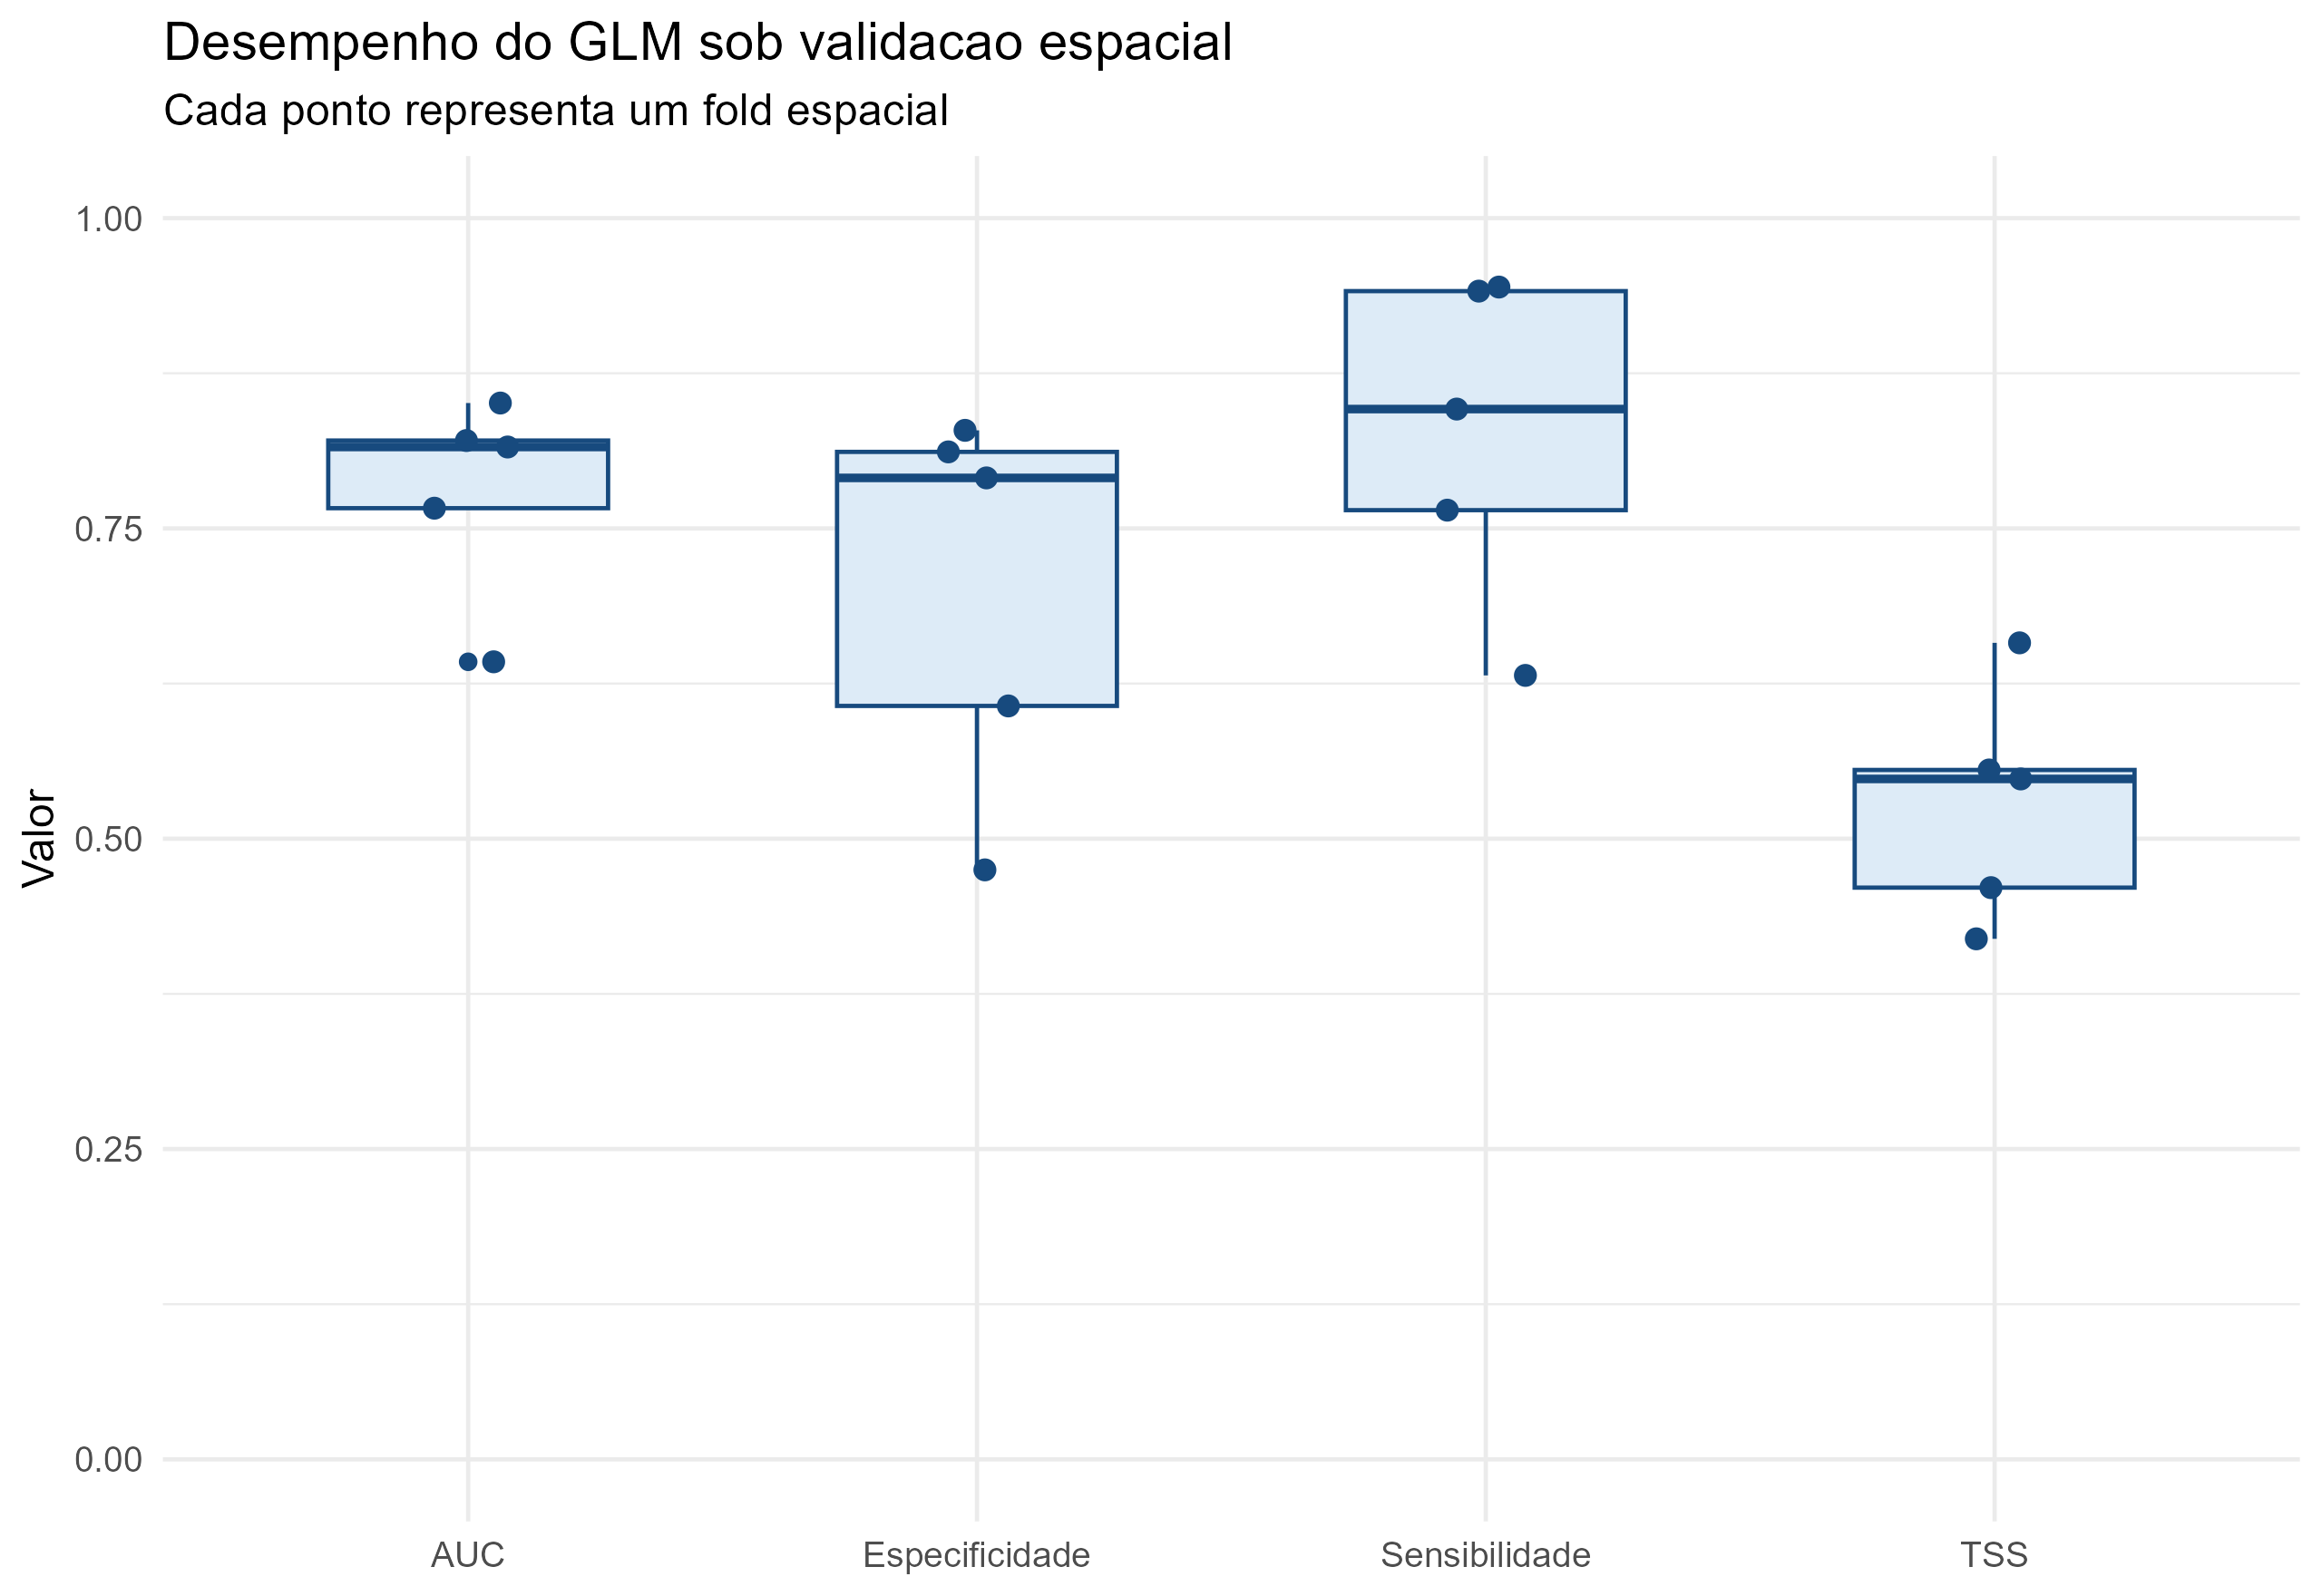
\includegraphics[width=0.88\textwidth]{figuras/unidade12/unidade12_validacao_espacial_glm.png}
\caption{Variation in GLM metrics among five spatial folds. Points are fold-specific results; the box is only a visual summary and does not replace inspection of individual values.}
\label{fig:unidade12-desempenho-espacial}
\end{figure}

The fits warned of probabilities numerically near zero or one. Although all
converged, 37 test predictions were extreme under the operational criterion
$\hat p\leq10^{-6}$ or $\hat p\geq1-10^{-6}$. This may indicate separation,
extrapolation, or excessive flexibility in quadratic terms and must be examined
before interpreting scores as calibrated probabilities. The results alone do
not establish superiority or inferiority relative to random validation; such a
comparison must hold model, data, preprocessing, and metrics constant.

\section{Spatial Sorting Bias}
Spatial sorting bias occurs when test presences are closer to training presences
than evaluation absences or background are. Even a geographic-distance-only
model may then achieve high AUC. Training--test distance inspection and null
models help reveal this bias \parencite{hijmans2012spatialsorting}.

\begin{decisao}[title={\faRoute\quad Methodological decision}]
Before calculating metrics, state whether the target is local interpolation,
geographic transfer, environmental transfer, or temporal projection. Construct
folds representing that prediction distance and use identical folds across
algorithms.
\end{decisao}

\section{Discrimination and Calibration}
Discrimination concerns ranking: do presences receive higher scores than
absences or background? Calibration concerns correspondence between predictions
and observed frequencies when such interpretation is valid. ROC curves and AUC
measure discrimination, not calibration. Reliability diagrams, calibration
intercept and slope, and proper scoring rules complement probabilistic evaluation
\parencite{vaughan2005testing,jimenezvalverde2013discrimination}.

\begin{conceito}[title={\faBalanceScale\quad A model can rank correctly but miss the magnitude}]
Models can rank sites similarly and have comparable AUC while producing values
with very different meanings and calibration. Discrimination does not authorize
interpreting suitability as occurrence probability.
\end{conceito}

\section{AUC and the ROC Curve}
The ROC curve relates sensitivity to $1-$specificity across thresholds. AUC is
the probability that a randomly selected presence receives a higher score than
a randomly selected background or absence:
\begin{equationbox}
\[AUC=P(\hat y_{presence}>\hat y_{background}).\]
\end{equationbox}
\begin{atencao}[title={\faExclamationTriangle\quad Limitations of AUC}]
With presence--background data, AUC depends on geographic extent, selected
background, sampling bias, and prevalence. A high value does not guarantee an
ecologically sound model.
\end{atencao}

\section{Sensitivity, Specificity, and TSS}
Sensitivity is the proportion of presences classified as suitable; specificity
is the proportion of absences or background classified as unsuitable.
\begin{equationbox}
\[Sensitivity=\frac{TP}{TP+FN}\]
\[Specificity=\frac{TN}{TN+FP}\]
\[TSS=Sensitivity+Specificity-1.\]
\end{equationbox}
TSS ranges from $-1$ to 1, with values nearer 1 indicating better binary discrimination.

\section{Kappa}
Kappa measures agreement between binary predictions and observations after
correcting for chance agreement, but is sensitive to prevalence and data distribution.
\begin{equationbox}
\[Kappa=\frac{p_o-p_e}{1-p_e},\]
\end{equationbox}
where $p_o$ is observed agreement and $p_e$ is chance-expected agreement.

\section{Boyce Index}
Boyce Index is useful for presence--background or presence-only models. It tests
whether presences occur preferentially where predicted suitability is higher
\parencite{hirzel2006evaluating}.
\begin{conceito}[title={\faBook\quad Boyce Index}]
Positive Boyce values indicate that presences concentrate in higher-suitability
classes, but the result depends on binning or smoothing choices and evaluation data.
\end{conceito}

\section{Integrated Evaluation Workflow}
\rscriptfile{scripts/unidade12/01_estrutura_pastas.R}
\rscriptfile{scripts/unidade12/02_preparar_predicoes_avaliacao.R}

\section{Calculating Metrics}
\rscriptfile{scripts/unidade12/03_calcular_metricas_modelos.R}
\begin{figure}[H]\centering
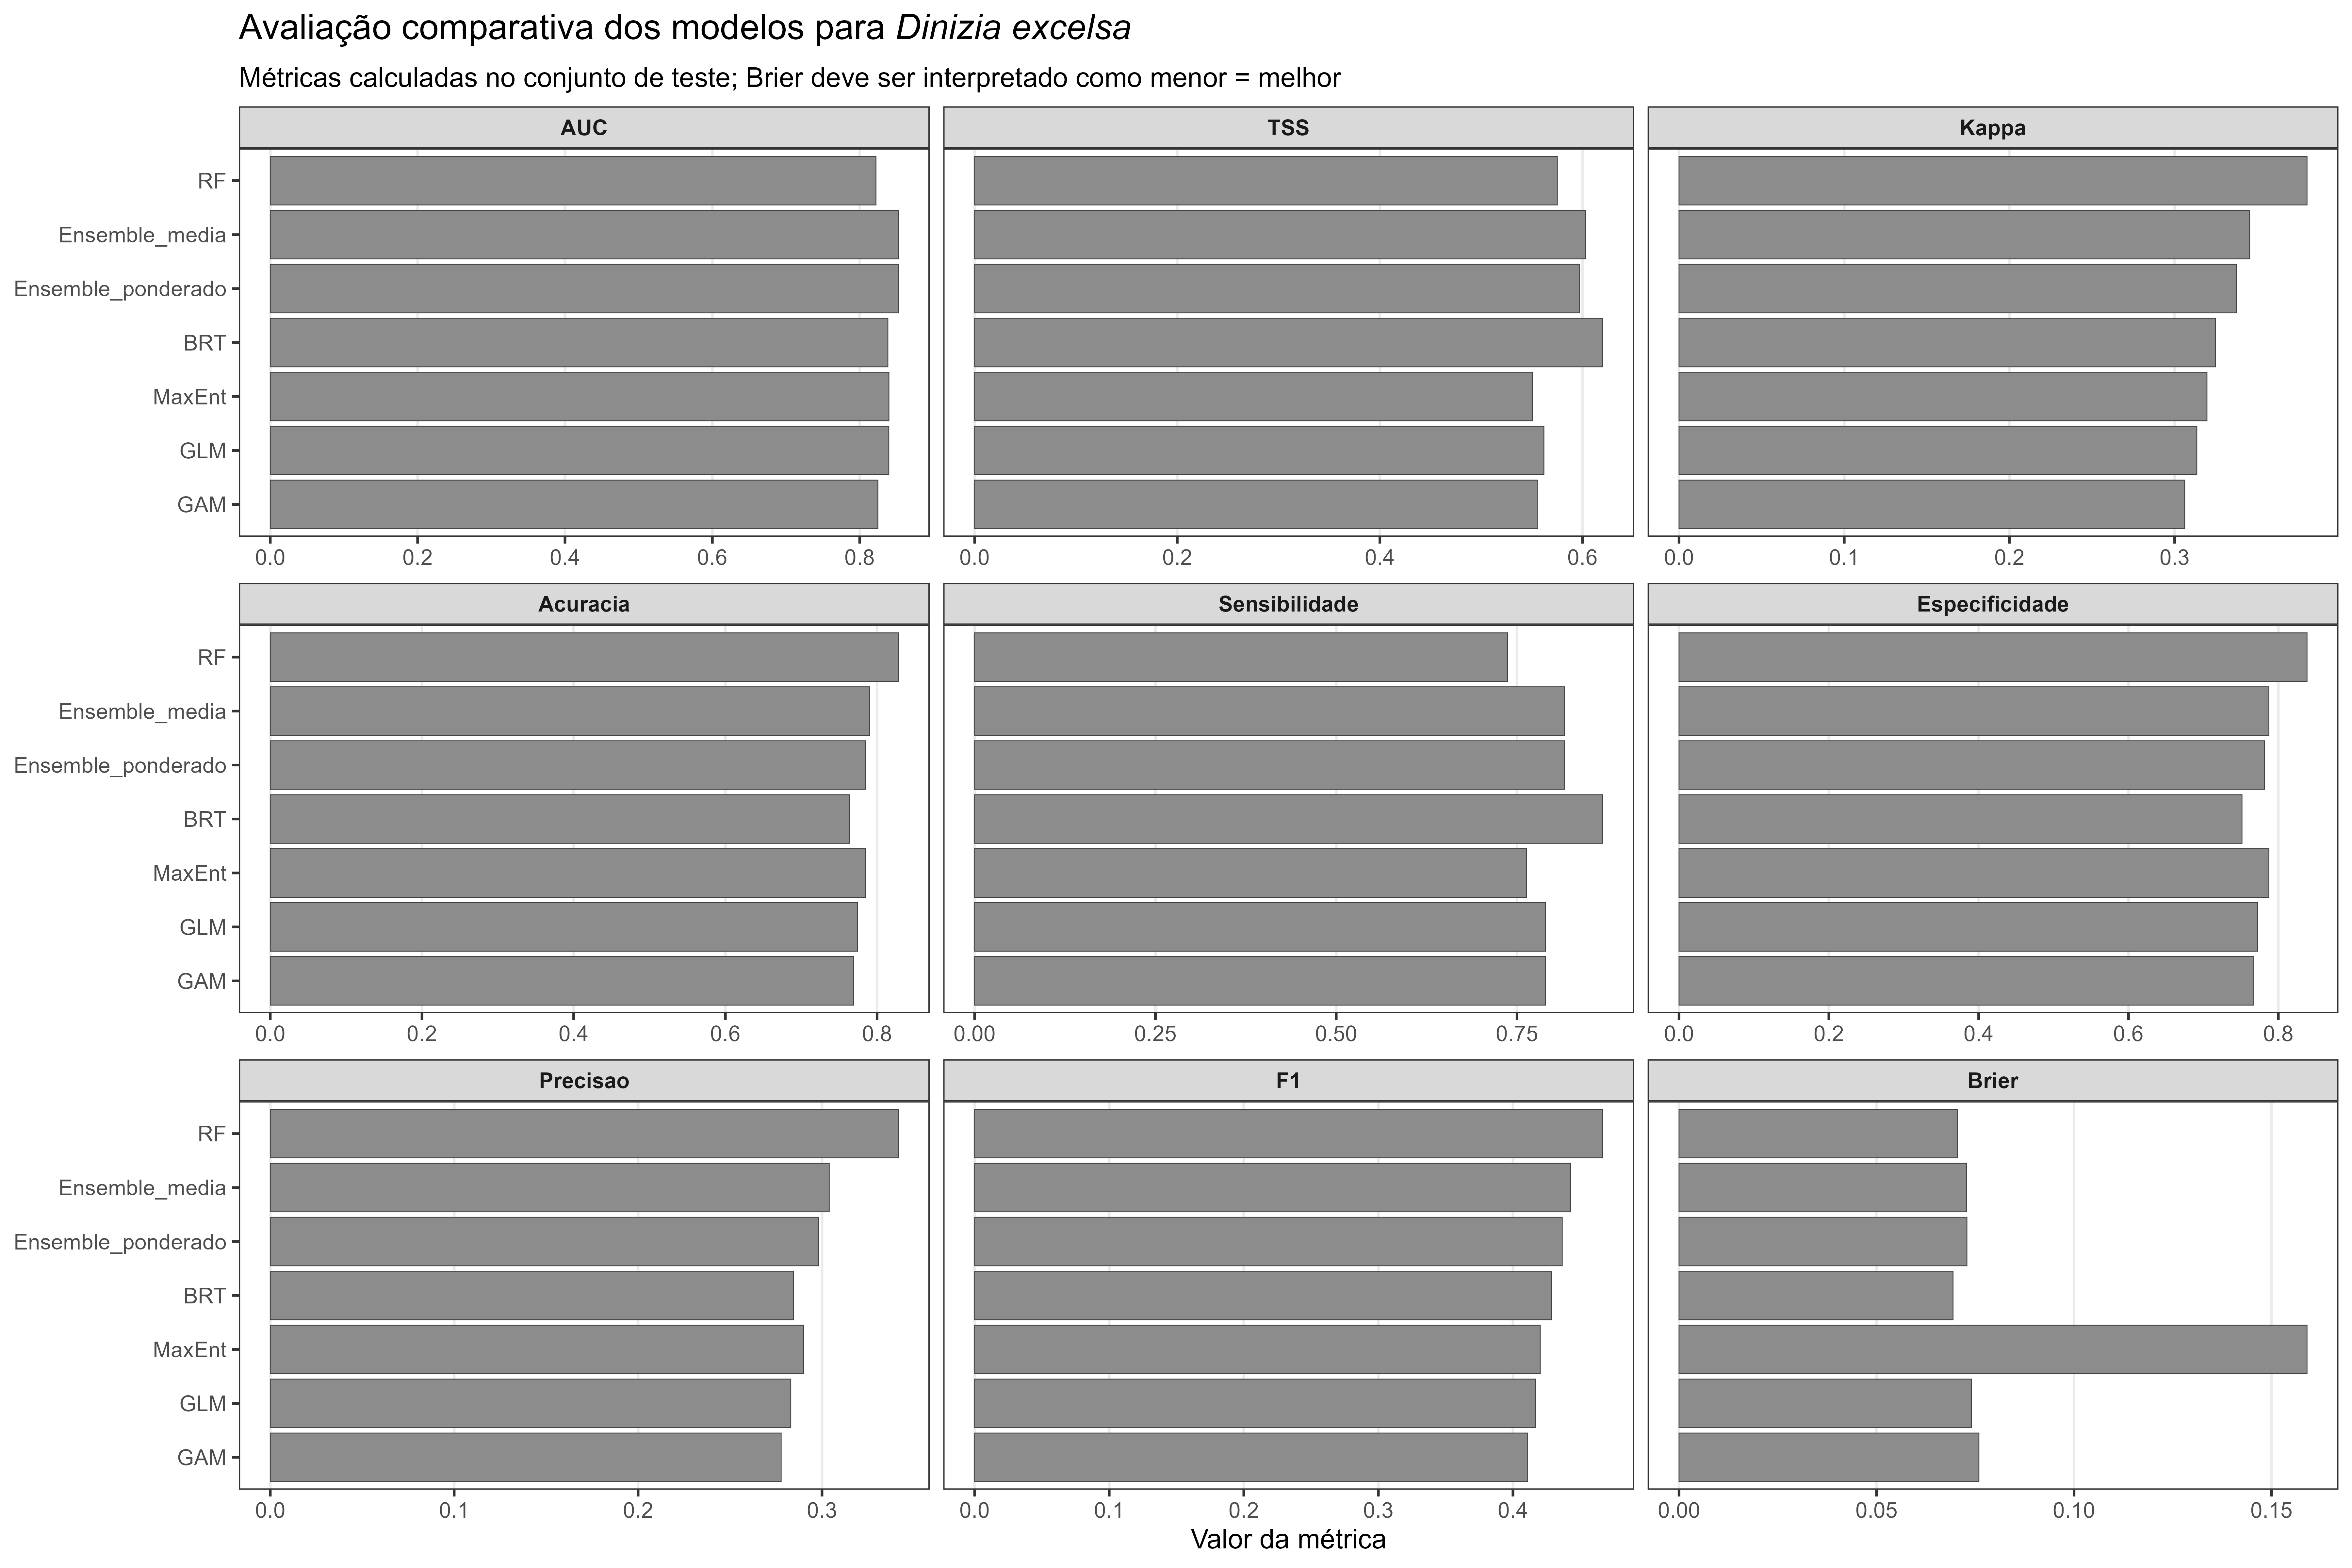
\includegraphics[width=0.95\textwidth]{figuras/unidade12/unidade12_comparacao_metricas.png}
\caption{Comparison of evaluation metrics for models fitted to \textit{Dinizia excelsa}.}\label{fig:unidade12_metricas}
\end{figure}

\section{Comparative ROC Curves}
\rscriptfile{scripts/unidade12/04_curvas_roc_comparativas.R}
\begin{figure}[H]\centering
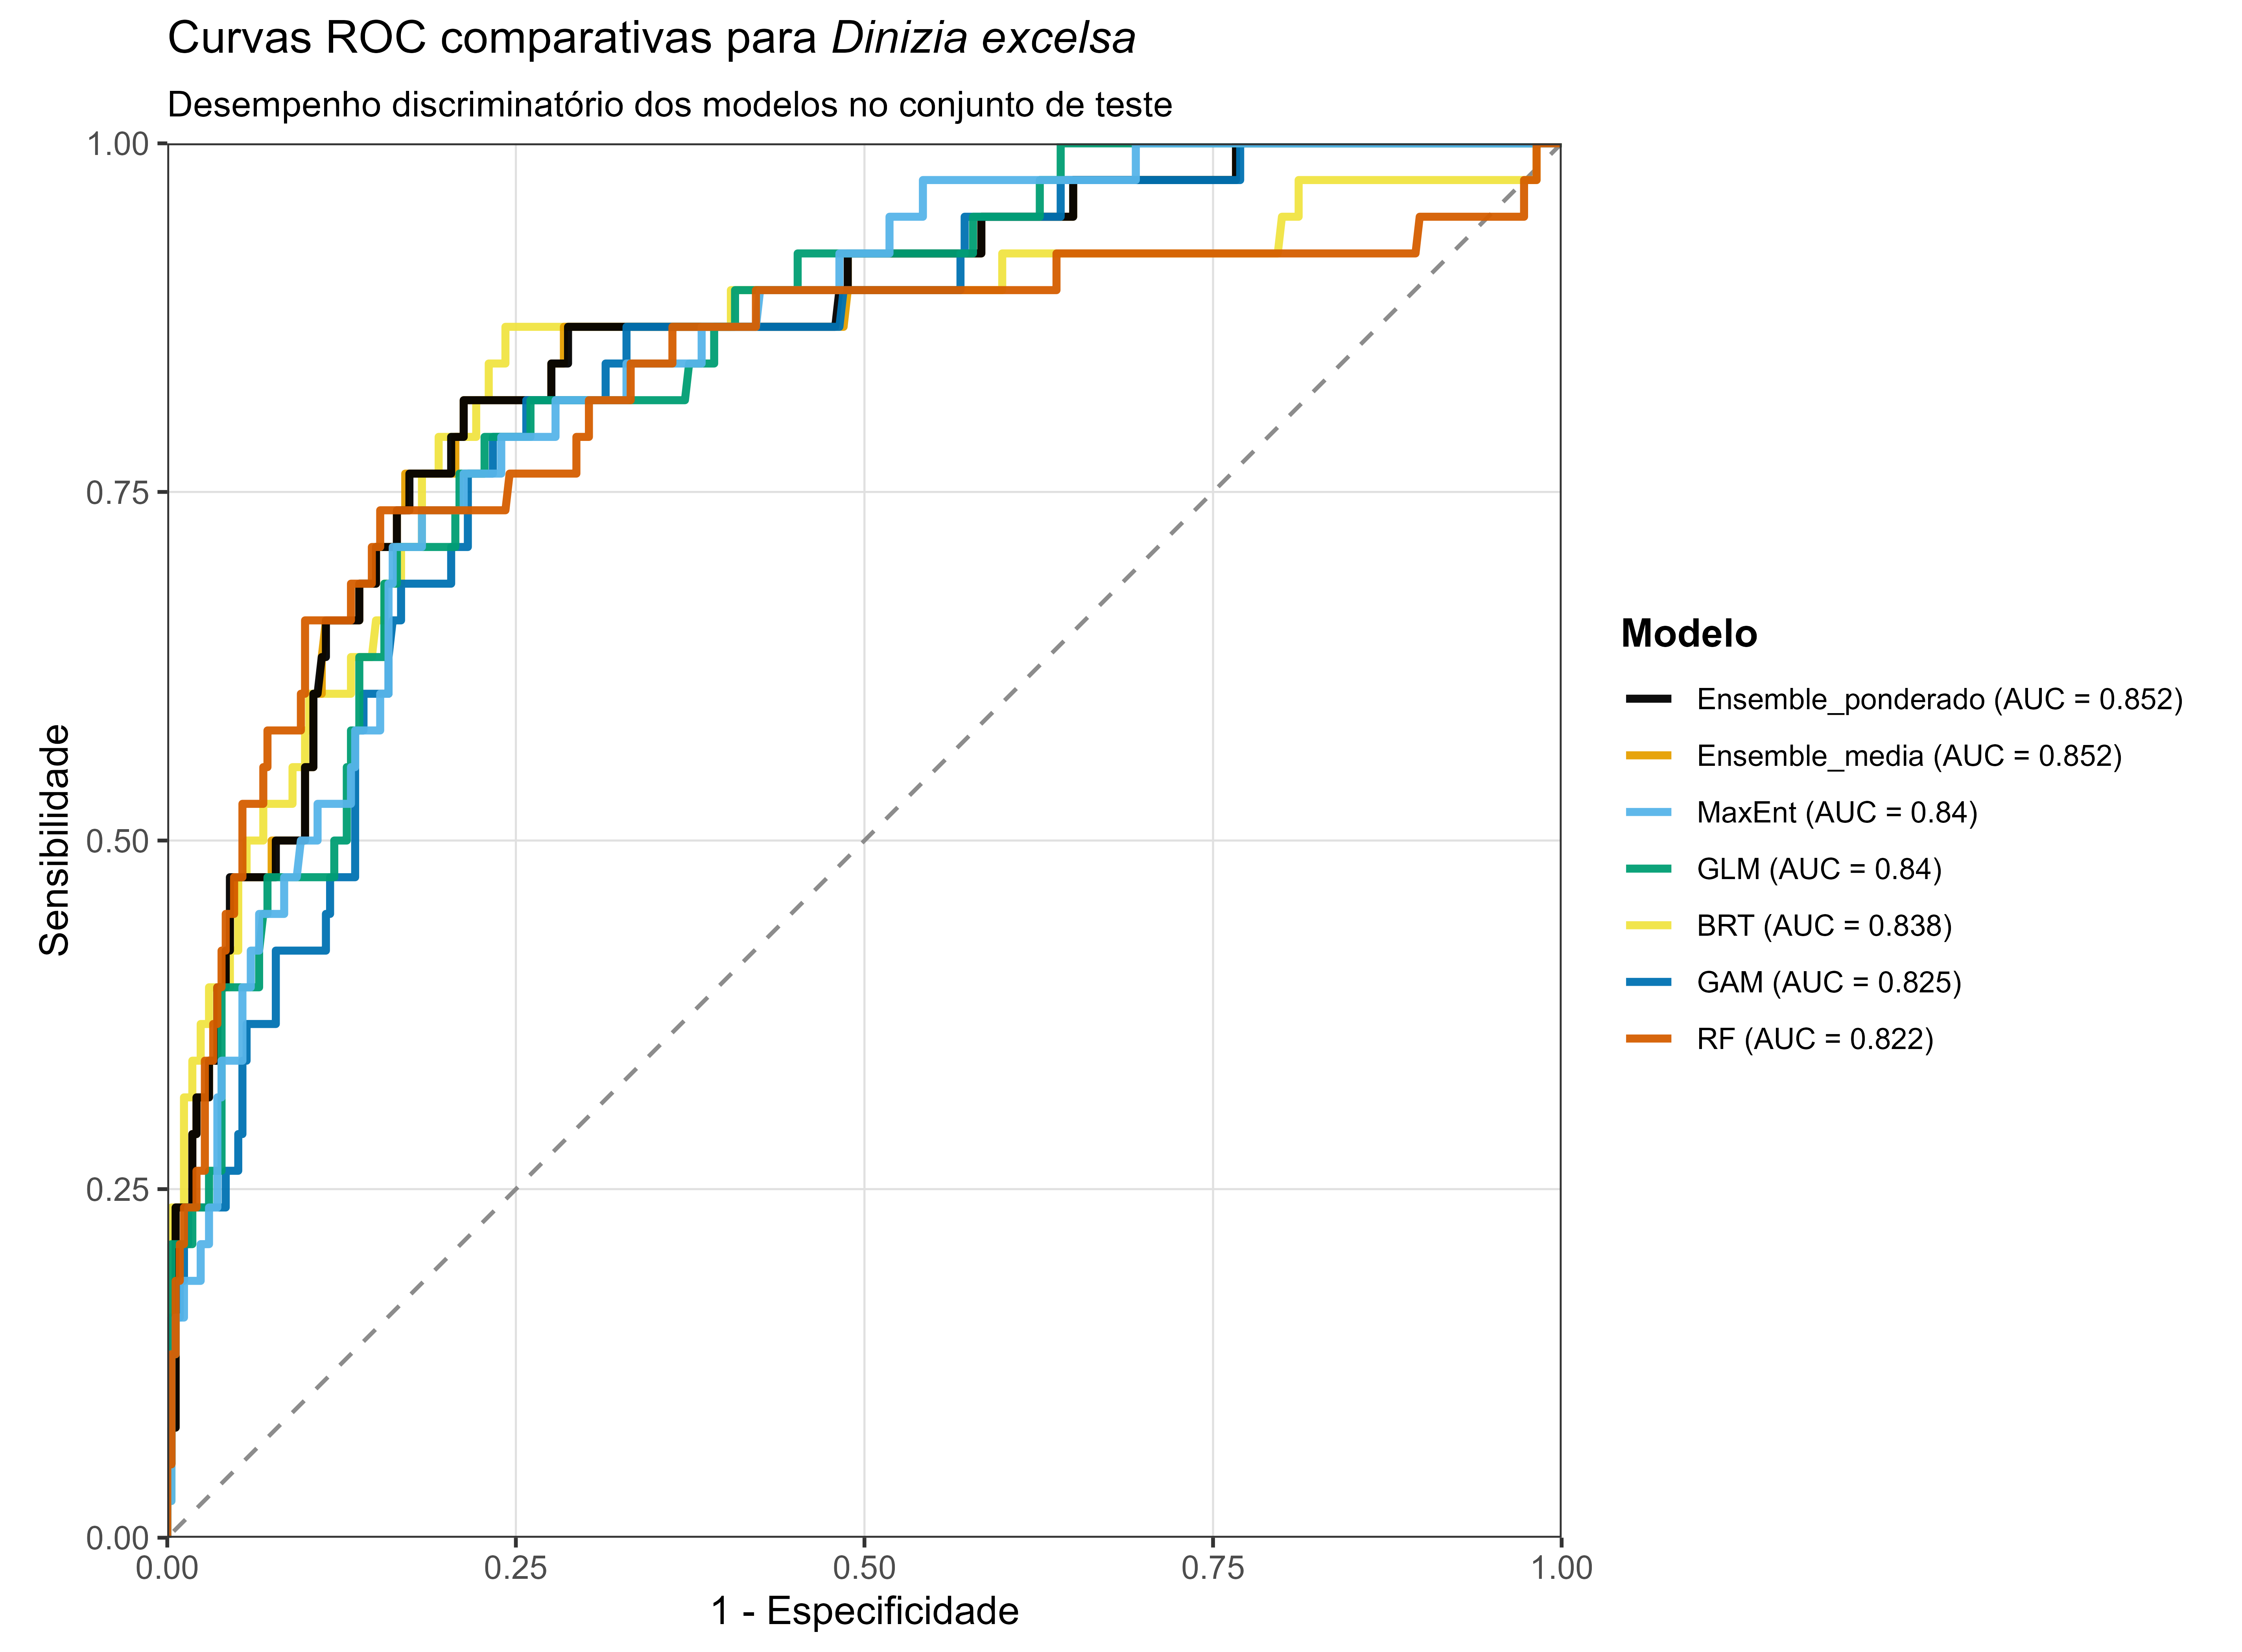
\includegraphics[width=0.86\textwidth]{figuras/unidade12/unidade12_curvas_roc_comparativas.png}
\caption{ROC curves for GLM, GAM, Random Forest, BRT, Maxent, and Ensemble.}\label{fig:unidade12_roc_comparativas}
\end{figure}

\section{Confusion Matrices}
\rscriptfile{scripts/unidade12/05_matrizes_confusao.R}
\begin{figure}[H]\centering
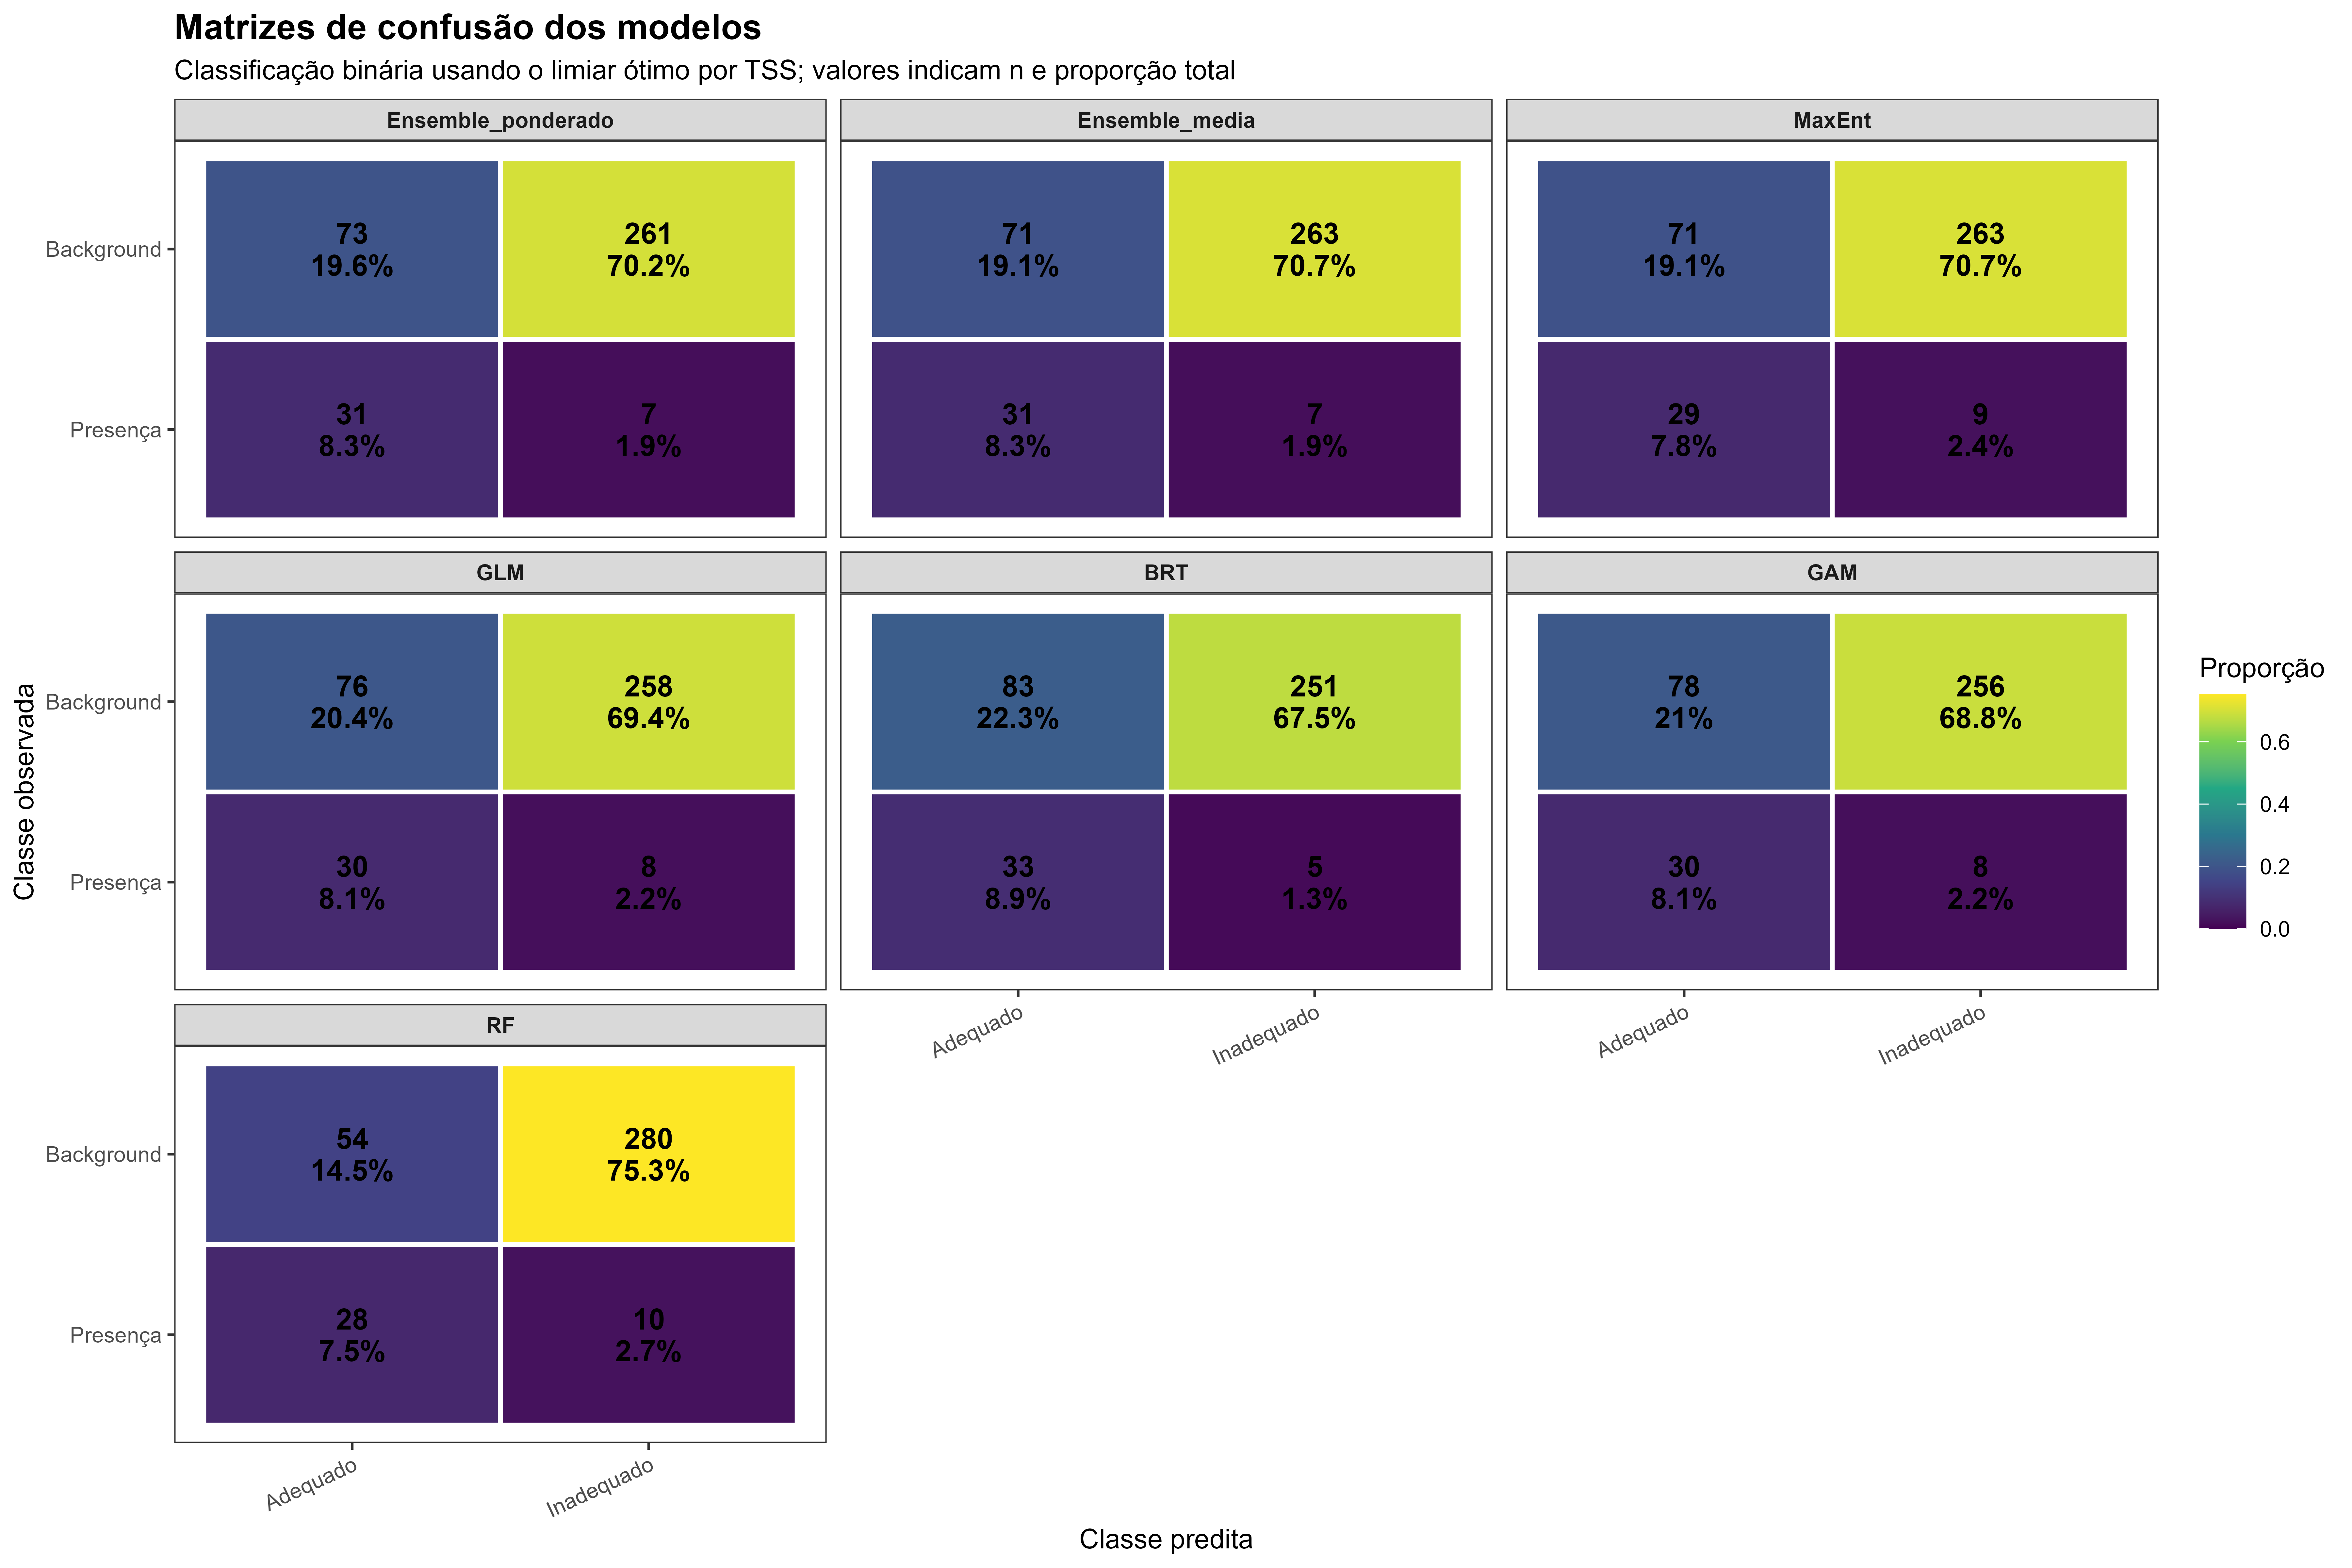
\includegraphics[width=0.95\textwidth]{figuras/unidade12/unidade12_matrizes_confusao.png}
\caption{Confusion matrices using TSS-selected thresholds.}\label{fig:unidade12_matrizes_confusao}
\end{figure}

\section{Binary Maps}
\rscriptfile{scripts/unidade12/06_mapas_binarios.R}
\begin{figure}[H]\centering
\includegraphics[width=0.98\textwidth]{figuras/unidade12/unidade12_mapas_binarios.png}
\caption{Binary suitability maps for \textit{Dinizia excelsa} using TSS-selected thresholds.}\label{fig:unidade12_mapas_binarios}
\end{figure}

\section{Comparative Synthesis}
\rscriptfile{scripts/unidade12/07_sintese_avaliacao.R}
\begin{figure}[H]\centering
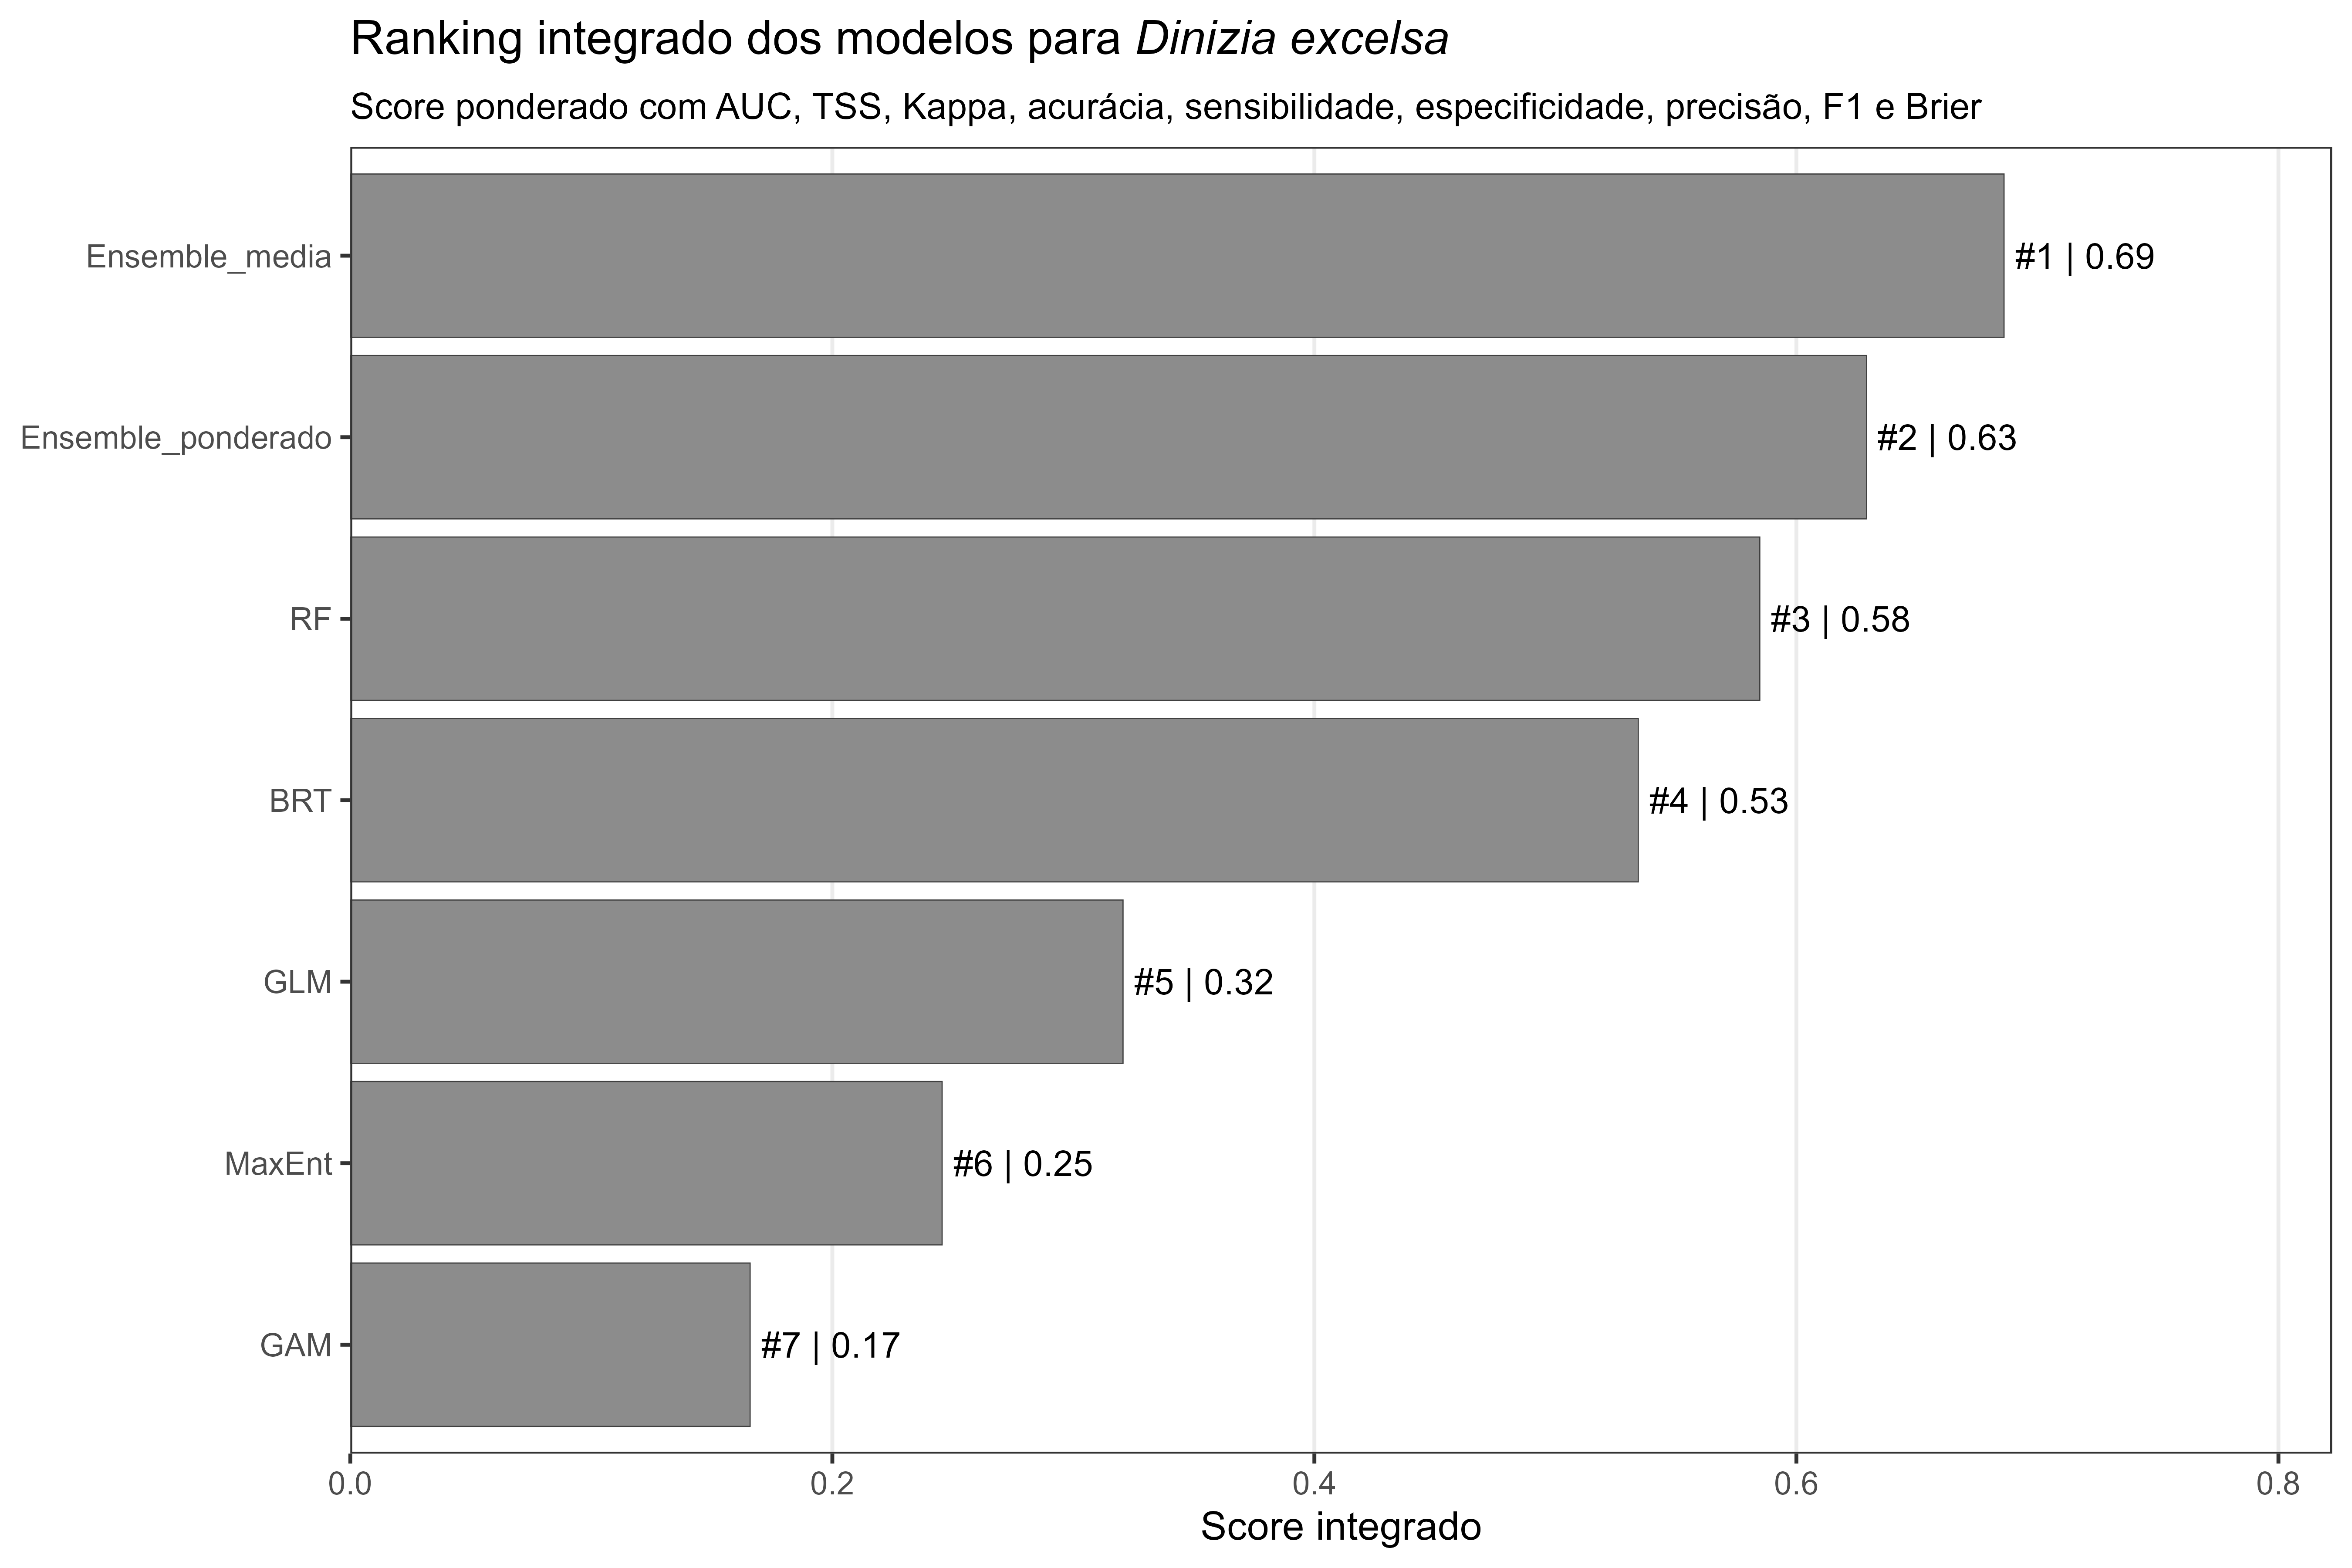
\includegraphics[width=0.95\textwidth]{figuras/unidade12/unidade12_ranking_modelos.png}
\caption{Comparative ranking using AUC, TSS, Kappa, sensitivity, specificity, and Boyce Index.}\label{fig:unidade12_ranking}
\end{figure}

\section{Complete Pipeline}
\rscriptfile{scripts/unidade12/08_pipeline_avaliacao.R}

\section{Chapter Summary}
Robust evaluation combines multiple metrics, independent validation, ecological
interpretation, response curves, uncertainty, and spatial plausibility.
\begin{conceito}[title={\faBook\quad Key message}]
No single metric validates an SDM. Robust evaluation combines continuous and
binary metrics, ecological interpretation, and spatial analysis of predictions.
\end{conceito}

\section{Review Exercises}
\subsection*{A. Concepts}
\begin{enumerate}
\item Explain the difference between AUC and TSS.
\item Why can AUC be problematic with presence--background data?
\item What do sensitivity and specificity mean?
\end{enumerate}
\subsection*{B. Interpretation}
\begin{enumerate}[resume]
\item Two models have the same AUC but different sensitivity. What are the consequences for identifying potentially suitable areas?
\item Performance decreases under spatial blocks. Interpret this without automatically rejecting the algorithm.
\item Explain the ecological meaning and one limitation of Boyce Index.
\end{enumerate}
\subsection*{C. Computation}
\begin{enumerate}[resume]
\item Recalculate metrics using identical folds and compare fold variation, not only means.
\item Construct spatial and environmental partitions; examine class balance in each fold.
\item Compare two thresholds and quantify changes in suitable area, omission, and commission.
\end{enumerate}
\subsection*{D. Critical Thinking}
\begin{enumerate}[resume]
\item Why should binary maps be interpreted cautiously?
\item How should validation differ between interpolation within Amazonia and projection to future climate?
\item Can a high-AUC presence--background model be called a well-calibrated occurrence-probability model? Justify.
\end{enumerate}

\subsection*{Mini-Project}
Select one \textit{Dinizia excelsa} algorithm. Compare random and spatial-block
evaluation while holding data, predictors, and metrics constant. Present the
fold map, training--test distance distribution, fold-specific metrics, and a
recommendation for interpolation and transfer.
